\chapter{\iflanguage{ngerman}{Technischer Hintergrund}{Technical background}}
\label{sec:methods}
\section{Hardware }

\subsection{Robot Platforms}
RSI used for communication with the robots
\subsubsection{KUKA KR 16-2}

\missingfigure{Please add some figures}

\subsubsection{KUKA KR 5}
\missingfigure{Please add some figures}





\section{\gls{ros2}}
The \gls{ros} is not an operating system in the classical sense \cite{quigley_ros_nodate, noauthor_ros_nodate}. Rather, ROS can be understood as a lightweight open-source collection of various software packages for robot development. It is a middleware that brings hardware abstraction, package management and communication between processes.\newline
\gls{ros} however, has its limitations regarding security, reliability in non-traditional environments, and support for large scale embedded systems. \gls{ros2} is the second redesigned generation of \gls{ros}. \gls{ros2} was developed from the ground up with the goal of overcoming these challenges \cite{macenski_robot_2022}.
\begin{figure}[htbp]
	\centering
	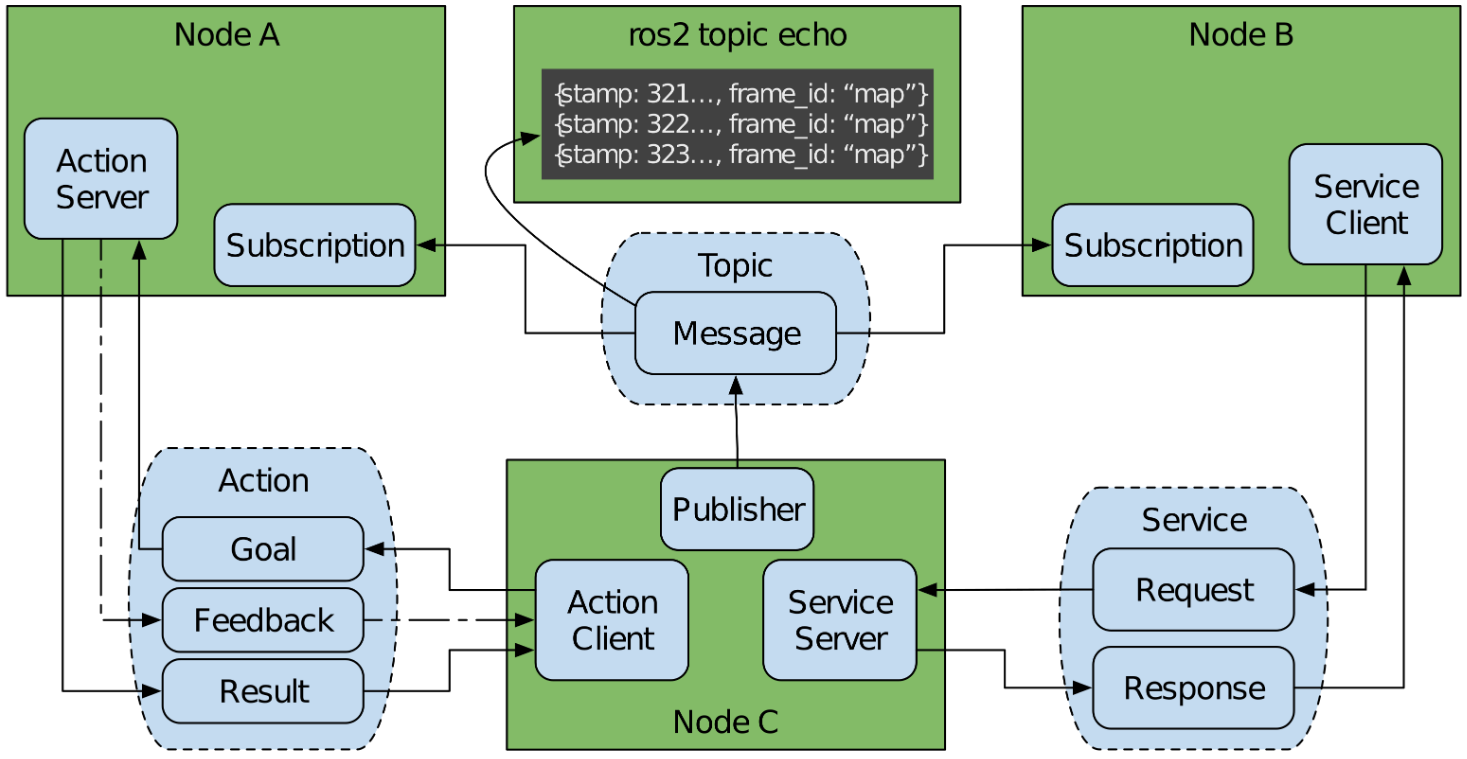
\includegraphics[width=1\textwidth]{Figures/c3/ros2_node_interfaces.png}
	\caption{The \gls{ros2} node interfaces \cite{macenski_robot_2022}.}
	\label{c3_fig_ros2_node_interfaces}
\end{figure}
\begin{figure}[htbp]
	\centering
	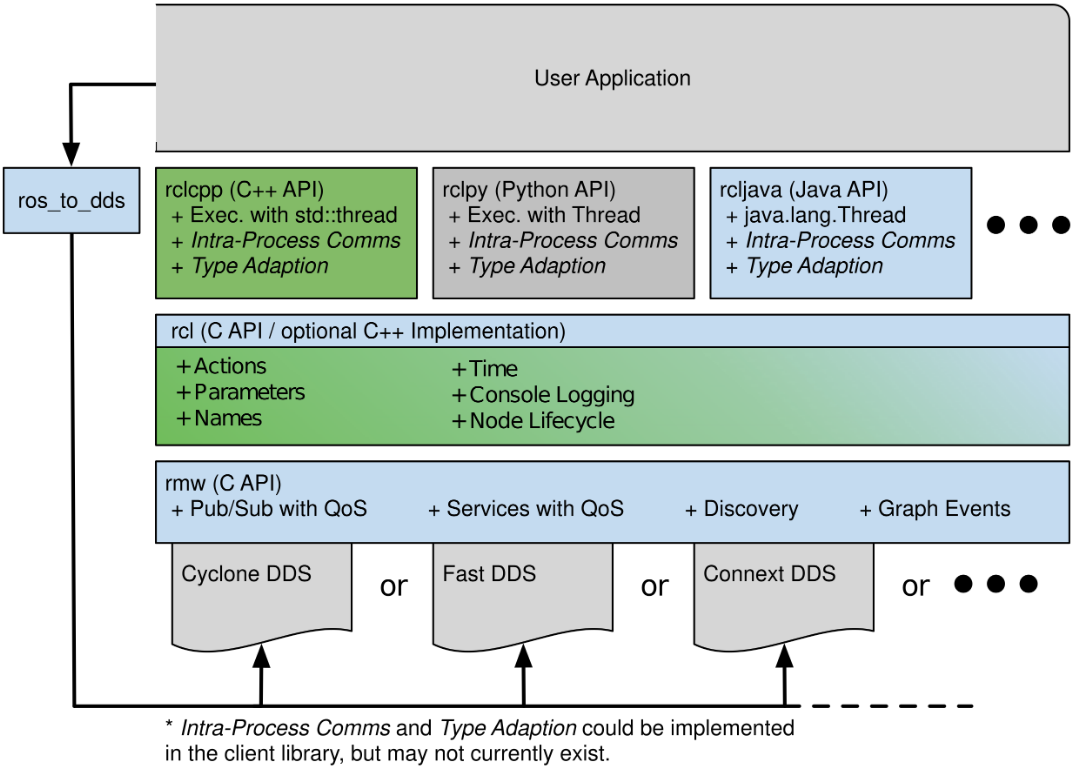
\includegraphics[width=1\textwidth]{Figures/c3/ros2_client_library_stack.png}
	\caption{The \gls{ros2} Client Library API Stack with the support of different \gls{dds} implementations shown \cite{macenski_robot_2022}.}
	\label{c3_fig_ros2_stack}
\end{figure}
ROS supports several programming languages such as Python, C++ and LISP. Written software can be divided thereby in dedicated nodes, so-called Nodes. A Node is here an independent process, which can communicate over Topics with other Nodes, via messages. It is possible for several nodes to connect to a topic. Besides the communication by means of this publisher-subscriber model, which implements a kind of "broadcast", there is another concept of synchronous message transmission. This is called service and provides a simple request-response protocol.\todoBetter{rewrite and adapt to ros2}







\section{The \gls{r2c} Control Framework}\label{ros2_control}
\Gls{r2c} is an open-source framework for real-time control, initially released for  \gls{ros2} Foxy. It is a rewrite of \gls{rc}, with the goal to simplify integration of new hardware and overcome some drawbacks present in \gls{rc} \cite{noauthor_welcome_nodate, magyar_getting_started_with_ros2_control_2021, magyar_ros2_control_the_future_of_ros_control_2021}. As shown in table \ref{c3_tab_r2c_repos} the framework comprises multiple repositories. It includes core functionality like management of controllers and hardware, as well as common controllers. Besides, it provides low-level tools for control theory and real-time control. \newline
A more detailed view of the internals of the \gls{r2c} framework is presented in figure \ref{c3_fig_ros2_control_uml}. As can be seen, the framework includes a controller manager. The controller is responsible for managing the controllers and connects them to the abstracted hardware. Additionally, it serves as entry-point for users and provides \gls{ros2} services through which the user can interact with the system. The controller manager has a resource manager, which in turn is responsible for storing and management of the hardware. The hardware is abstracted through interfaces \newline
The control loop itself consist of three steps:
\lstset{language=C++,basicstyle=\scriptsize}
\begin{lstlisting}[caption=Pseudo code for the control loop.]
// creat controller manager with an rclcpp::executor
auto cm = 
    std::make_shared<controller_manager::ControllerManager>(executor, cm_node_name);
while (rclcpp::ok())
{   
    // calculated meassured_period
    // execute update loop
    cm->read(cm->now(), measured_period);
    cm->update(cm->now(), measured_period);
    cm->write(cm->now(), measured_period);
    //sleep until next iteration
}
\end{lstlisting}\label{c3_code_control_loop}

\begin{figure}[htbp]
	\centering
	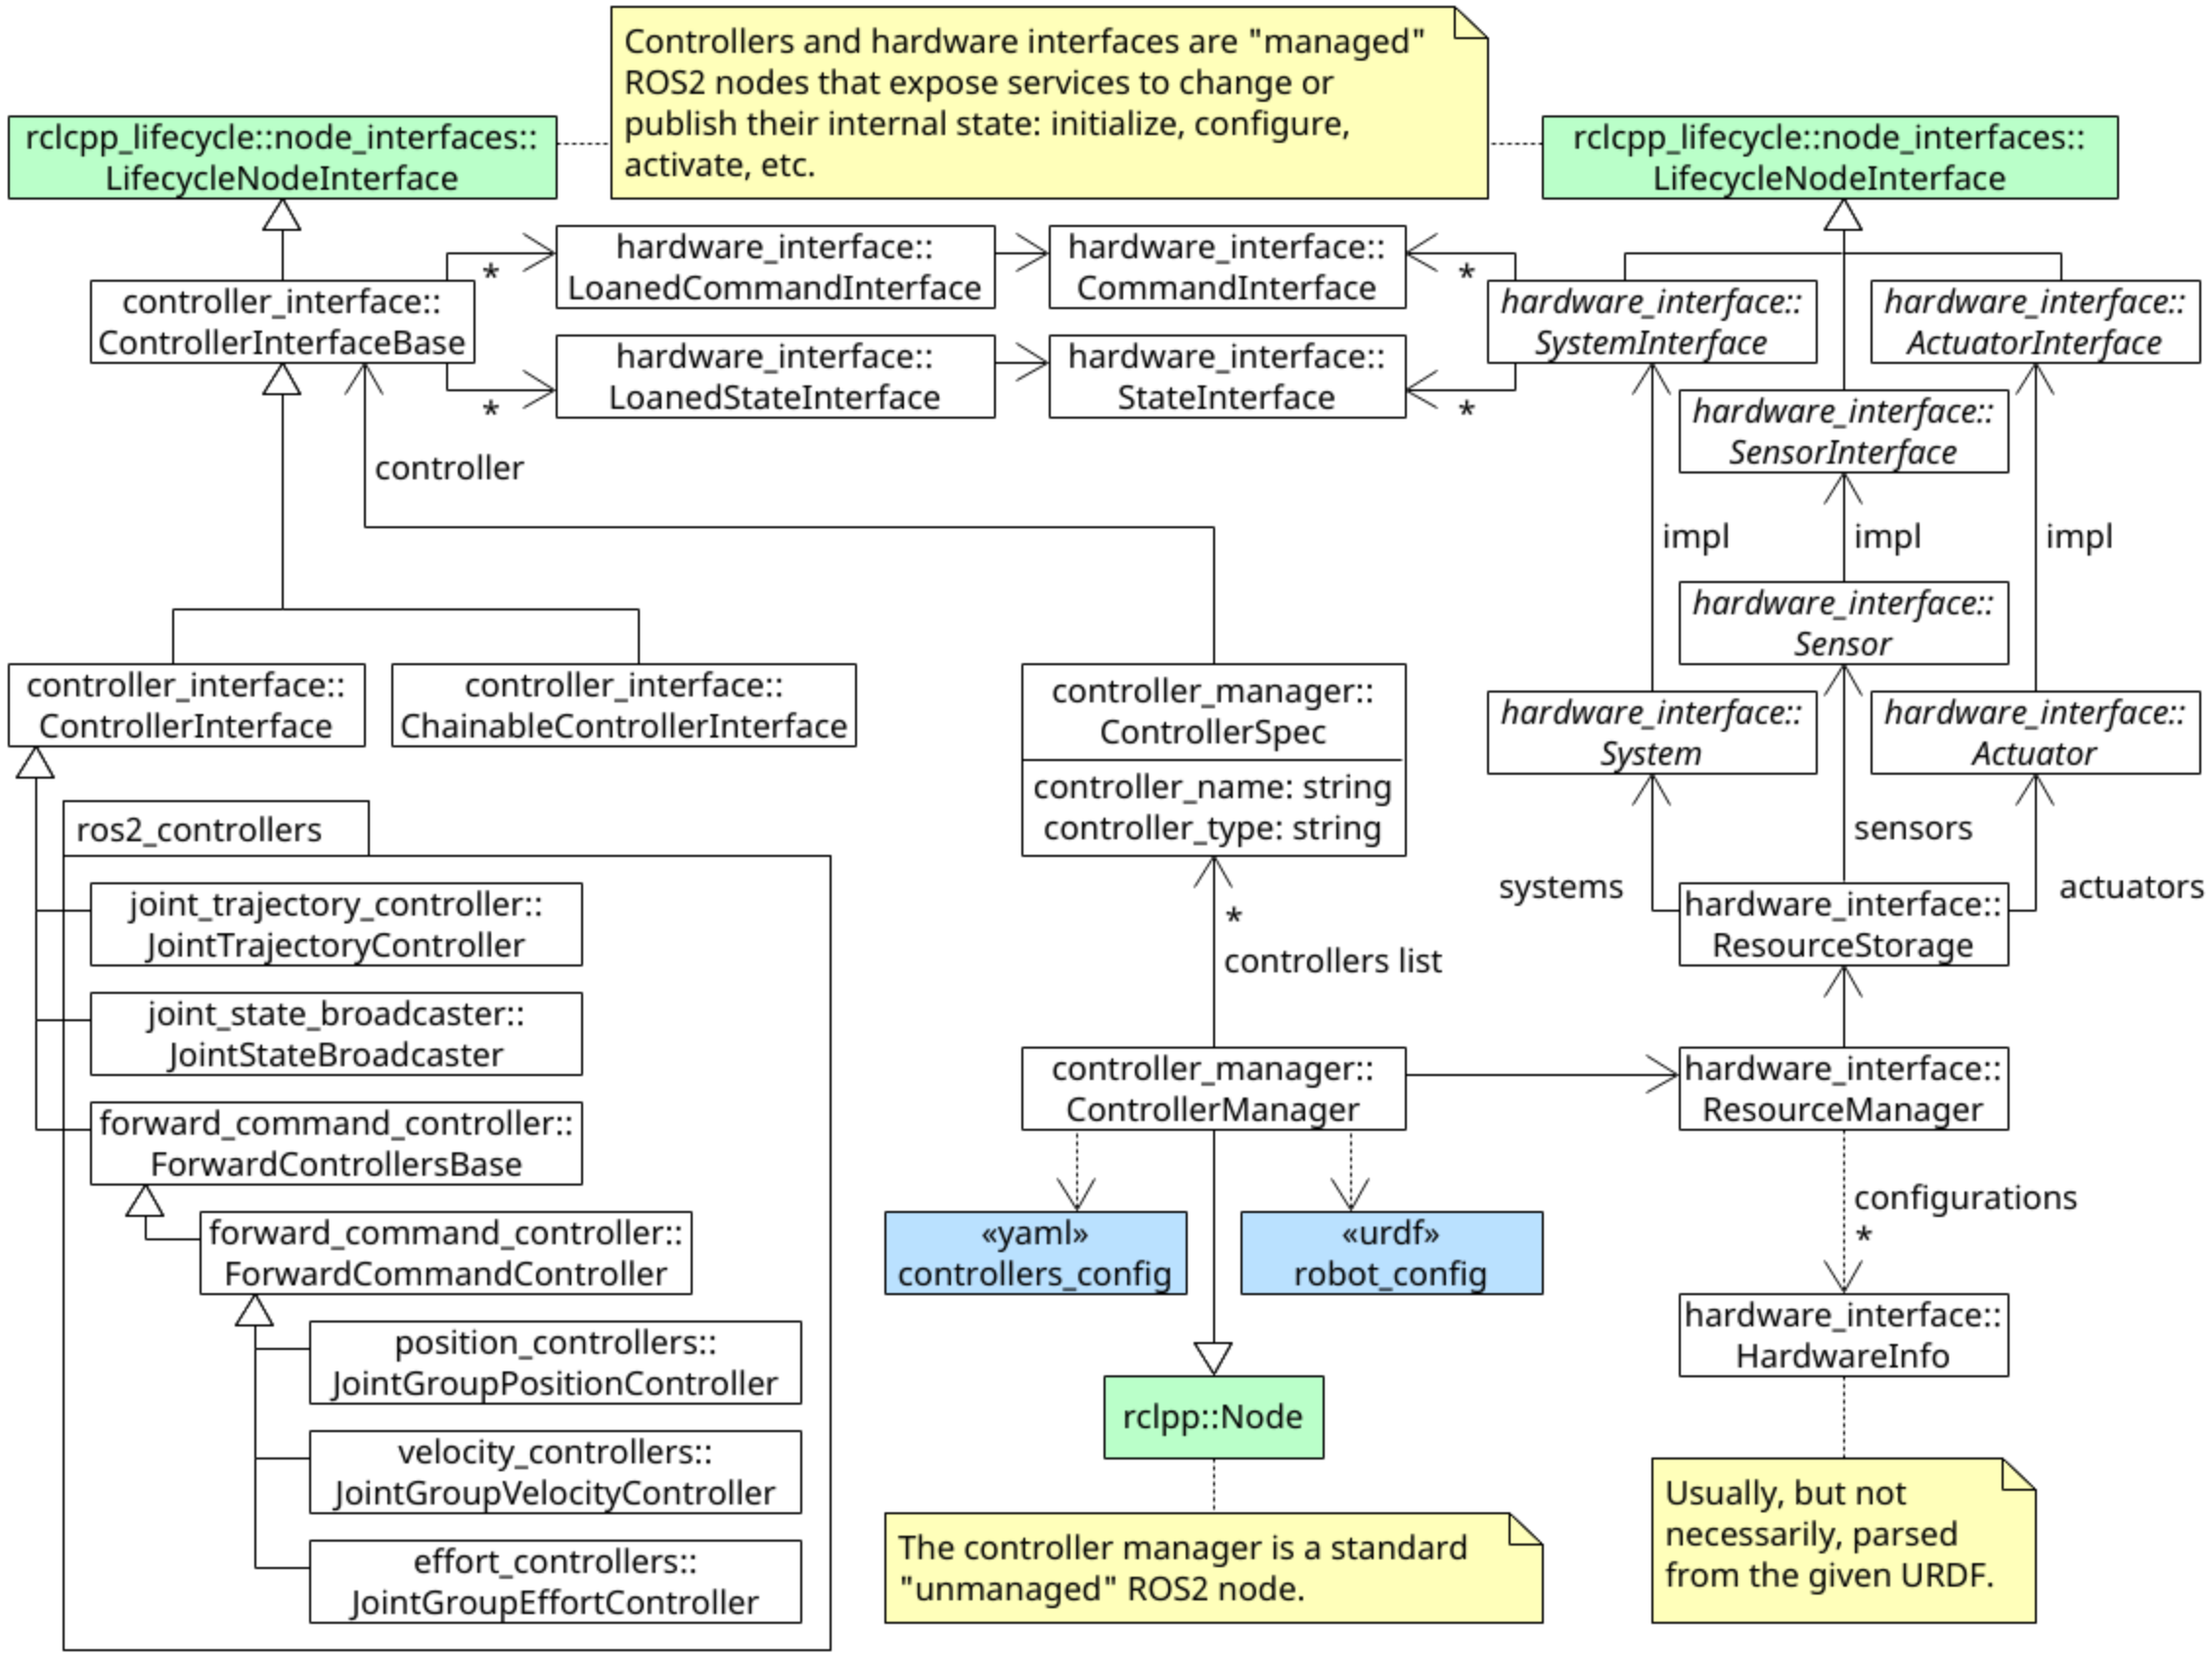
\includegraphics[width=1\textwidth]{Figures/c3/ros2_control_uml.png}
	\caption{UML diagram of the most important classes and interfaces in the \gls{r2c} framework. Picture taken from \cite{noauthor_welcome_nodate}. }
	\label{c3_fig_ros2_control_uml}
\end{figure}\todoBetter{Replace with own figure}

\begin{table}[htbp]
    \centering
\begin{tabular}{ |c|c| }
\hline
\multicolumn{2}{|c|}{\gls{r2c} repositories} \\
\hline
Repository & Description  \\
\hline
\hline
\href{https://github.com/ros-controls/ros2_control}{ros2\_control} 
 & \begin{minipage}{11cm}
	 \vskip 8pt
		 Core functionality like controller manager, resource manager, interfaces for hardware abstraction, and more.
	 \vskip 8pt
	\end{minipage}  \\
\href{https://github.com/ros-controls/ros2_controllers}{ros2\_controllers}  & \begin{minipage}{11cm}
	 \vskip 8pt
		 Collection of commonly and widely used controllers like forward command controller, joint trajectory, \dots
	 \vskip 8pt
	\end{minipage}  \\
\href{https://github.com/ros-controls/control_toolbox}{control\_toolbox}  & \begin{minipage}{11cm}
	 \vskip 8pt
		Control theory implementations (e.g. PID) used by controllers.
	 \vskip 8pt
	\end{minipage}  \\
\href{https://github.com/ros-controls/realtime_tools}{realtime\_tools}  & \begin{minipage}{11cm}
	 \vskip 8pt
		 Toolkit for real-time use. It includes e.g. real-time buffers and real-time publishers.
	 \vskip 8pt
	\end{minipage}  \\
\href{https://github.com/ros-controls/control_msgs}{control\_msgs}   & \begin{minipage}{11cm}
	 \vskip 8pt
		 Common messages used within the framework.
	 \vskip 8pt
	\end{minipage}  \\
\hline
\end{tabular}
    \caption{Overview of the repositories the \gls{r2c} framework includes.}
    \label{c3_tab_r2c_repos}
\end{table}



\subsection{Real-Time Capability of \gls{ros2} and \gls{r2c}}

\subsection{Controlling Multiple Robots with \gls{r2c}}




\section{Echtzeitfähige Netzwerke}


\subsection{Fast DDS}


\subsection{Cyclon DDS}



